\documentclass[12pt]{article}
\usepackage{amsmath, amsthm, amssymb, graphicx}
\title{Non-Accidental Consciousness: A Formal Argument}
\author{Prepared by Caleb Archer}
\date{\today}

\begin{document}
\maketitle

\begin{abstract}
This paper argues that the accidental emergence of conscious life and 
complementary sustaining ecosystems has probability zero under unguided processes. 
The argument distinguishes awareness from consciousness, formalizes the zero-probability 
proof, and addresses objections from emergent materialism and the anthropic principle.
\end{abstract}

\section{Introduction}
We explore the distinction between awareness and consciousness and the 
implications for evolution and ecosystem co-dependence.

\section{Definitions}
\input{../docs/01_definitions.md}

\section{Zero-Probability Argument}
\input{../docs/02_zero_probability_argument.md}

\section{Formal Proof}
\input{../docs/03_formal_proof.md}

\section{Counterarguments}
\input{../docs/04_counterarguments.md}

\section{Philosophical Defense of P1/P2}
\begin{itemize}
\item Consciousness cannot arise from unconscious substrate
\item Awareness is prerequisite for consciousness
\item References: Chalmers, Whitehead, Strawson, Lanza
\end{itemize}

\section{Diagram}
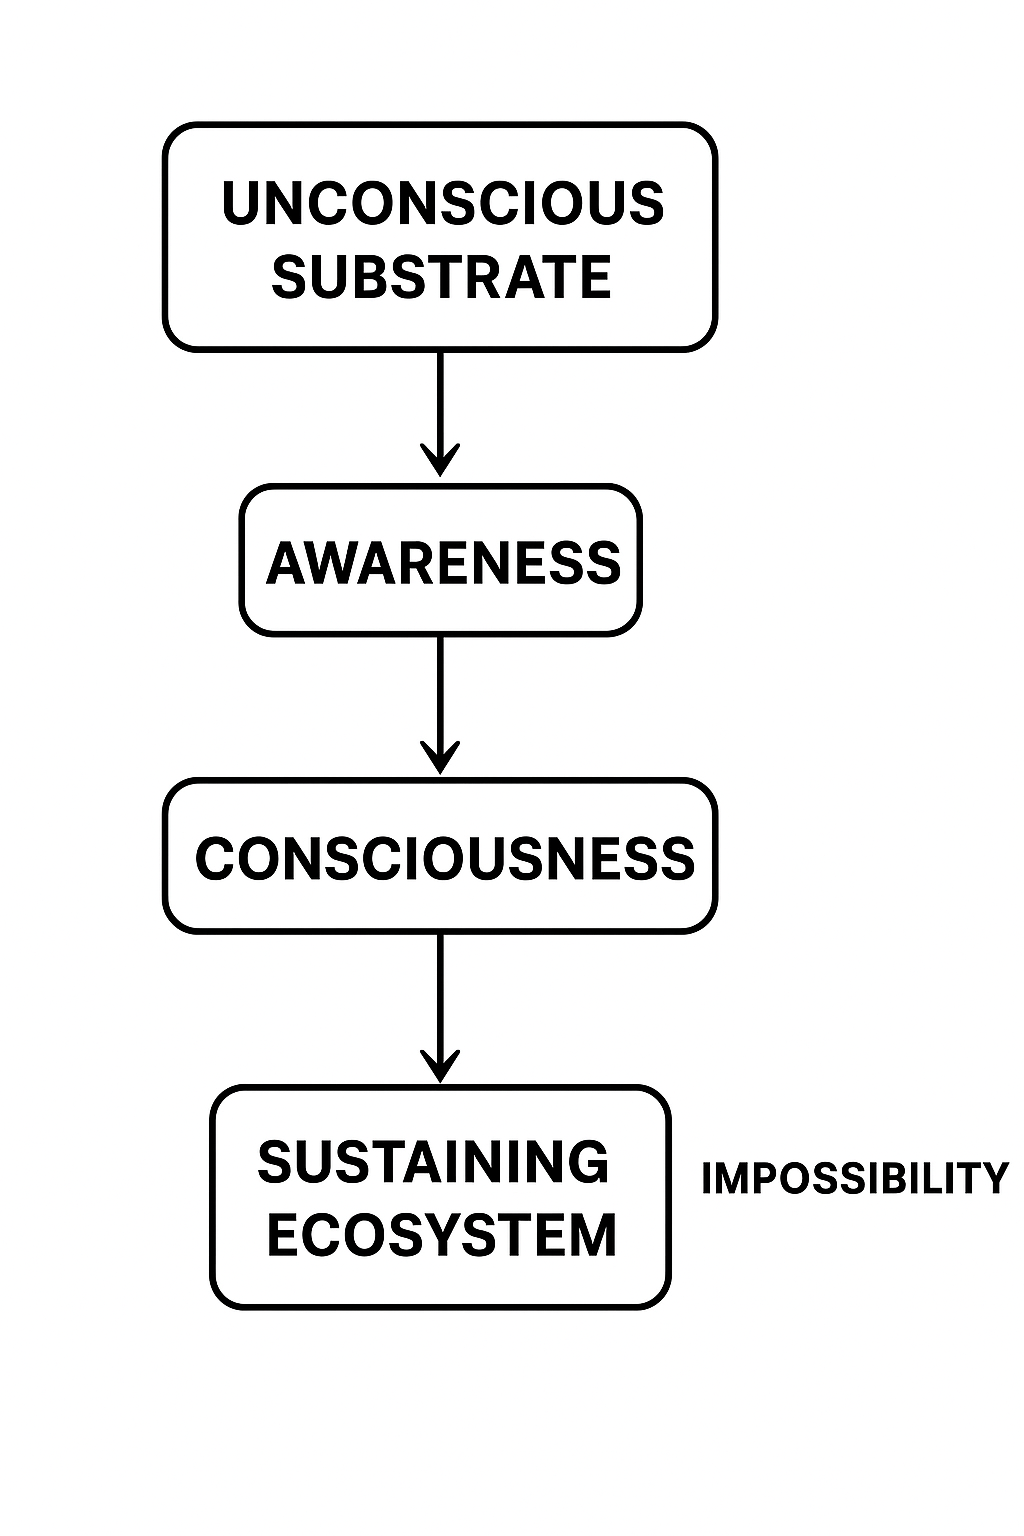
\includegraphics[width=\textwidth]{../diagrams/impossibility_flowchart.png}

\section{Conclusion}
Consciousness and sustaining ecosystems cannot emerge accidentally. They are 
either fundamental or require non-accidental processes.
\end{document}
